\section{Introduction}

\begin{itemize}
\item Making sense of data-driven claims is hard, even if the evidence base (code/data) is open
\item We see this in peer review, misinformation, retracted papers, …
\end{itemize}

\begin{figure}[h]
   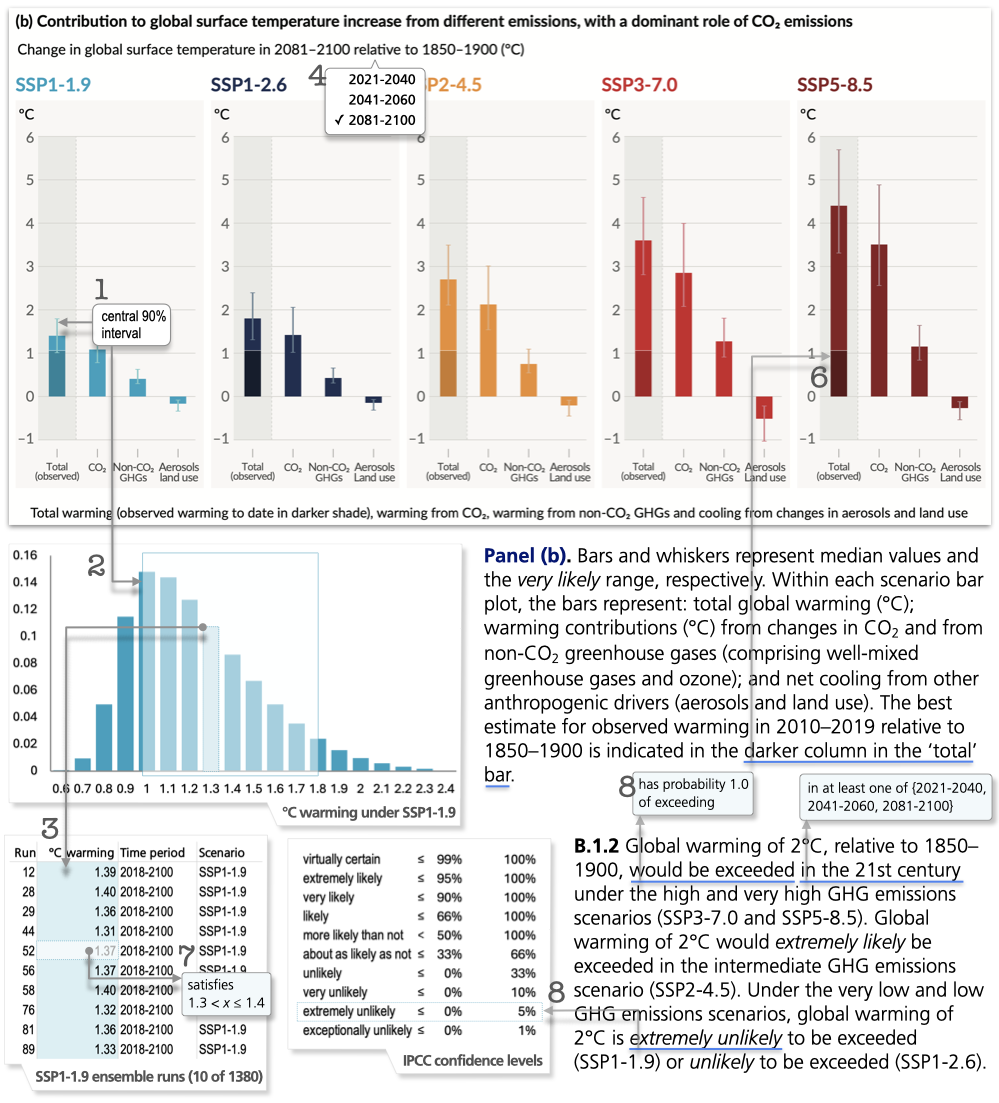
\includegraphics[width=0.9\textwidth]{fig/ipcc-mockup.png}
   \caption{Mockup of end-user transparency features (numbered 1 to 8)}
   \label{fig:ipcc-mockup}
\end{figure}

\subsection{Self-Certifying Text}

\begin{itemize}
\item Introduce basic idea, as complementary to transparent visualisations
\end{itemize}

\subsubsection{Use cases}
Two potential scenarios for this sort of technology:

\paragraph{Authoring transparent text.} Someone authoring content for an online article, wants to create text
linked to raw data (and derivative data such as charts or tabular summaries), so that the evidence base for
the claims made in the text can be explored \emph{in situ}, by interacting with the text.

\paragraph{Interpreting text after the fact.} Someone reading textual claims derived from open data (e.g. a
scientific paper or climate report), wants to retroactively link the text to queries over the available data
and gradually ``rationally reconstruct'' the relationship between the claims in the paper and the evidence
base. Perhaps just to aid their own comprehension, or to provide some kind of justified peer review.

\vspace{2mm}
\noindent Here we focus on the first one because the second one requires a certain amount of additional setup.

\subsubsection{Target idioms of natural language}

NLP aspect of the problem is potentially a big problem space in itself. We will restrict interest to certain
idiomatic uses of natural language in making/justifying scientific claims. Examples:



\begin{itemize}
\item quantitative expressions
\begin{itemize}
   \item pure numerical values
   \item percentages
   \item rounded or normalised numbers
\end{itemize}
\item aggregation
\begin{itemize}
   \item average
   \item totals
   \item count
\end{itemize}
\item trends
\begin{itemize}
   \item comparisons
   \item ranks
\end{itemize}
\item graded Adjectives (e.g.~\emph{virtually certain}, \emph{exceptionally unlikely})
\item references to visual elements and their parts (mereology)
\end{itemize}

\begin{table}[!ht]
   \centering
   \tiny
   \renewcommand{\arraystretch}{1.5}
   \begin{tabular}{p{1.5cm}p{1.5cm}p{5cm}p{4cm}}
      \toprule
      \textbf{Category} & \textbf{Type} & \textbf{Example} & \textbf{Result} \\
      \midrule
      \rowcolor{green!20}
      Quantitative expressions & Pure numerical values &
      \begin{lstlisting}[language=Fluid]
            (findWithKey' "model" "LSTM" tableData).time\_s
      \end{lstlisting}
      & 67 \\
      \rowcolor{green!20}
      Quantitative expressions & Percentages &
      \begin{lstlisting}[language=Fluid]
         "The Energy Sector accounts for total methane emissions of", (record.emissions / sum(map (fun x -> x.emissions) (getByYear year tableData))) * 100, "in 2030"
      \end{lstlisting} &
      The Energy Sector accounts for total methane emissions of 52.80\% in 2030.\\
      \rowcolor{green!20}
      Quantitative expressions & Rounded or normalised numbers & ~ & ~ \\
      \rowcolor{green!20}
      Aggregation & Average &
      \begin{lstlisting}[language=Fluid]
         The average methane emissions for the year 2030 is, (sumEmissions year tableData / length records)
      \end{lstlisting}
      & The average methane emissions for the year 2030 is 13.51 \\
      \rowcolor{green!20}
      Aggregation & Totals &
      \begin{lstlisting}[language=Fluid]
         "The total methane emissions for the year 2030 is", (sumEmissions year tableData), "for Agriculture"
      \end{lstlisting} &
      The total methane emissions for the year 2030 is 37.74 for Agriculture \\
      Aggregation & Count &  ~ & ~ \\
      \rowcolor{green!20}
      Trends & Comparisons &
      \begin{lstlisting}[language=Fluid]
         trendWord (findWithKey' "model" "BiLSTM" tableData).time\_s (findWithKey' "model" "LSTM" tableData).time\_s "growing from" "shrinking to" "equal to"
      \end{lstlisting}
      & growing from \\
      \rowcolor{green!20}
      Trends & Ranks &
      \begin{lstlisting}[language=Fluid]
         let pos = findIndex "model" "CNN" (insertionSort cmpTime tableData) in rankLabel "lowest" pos
      \end{lstlisting}
      & lowest \\
      Adjectives & Graded adjectives  &  ~ & ~ \\
      References to visual elements and their parts (mereology) & ~ & ~ & ~ \\
      \bottomrule
   \end{tabular}
   \caption{Example expressions generated by the Authoring Assistant, classified by type. In green, the expression is already tested.}
   \label{tab:fluid_examples}
   \renewcommand{\arraystretch}{1.0}
\end{table}

\subsection{Contributions}

\begin{itemize}
\item Design and proof-of-concept implementation of AI-assisted workflow for authoring transparent text
(\secref{authoring-workflow})
\item Empirical evaluation of how effective current LLMs are at providing the ``AI-assisted'' part
\end{itemize}
